\documentclass{article}

\usepackage{graphicx}
\usepackage{tikz}
\usepackage{tikzsymbols}
\usetikzlibrary{calc,patterns,shapes.geometric}
\pagestyle{empty}
\usepackage[margin=0pt]{geometry}
\geometry{papersize={14in,12in}}

\def\centerarc[#1](#2)(#3:#4:#5){\draw[#1] ($(#2)+({#5*cos(#3)},{#5*sin(#3)})$) arc (#3:#4:#5);}

\begin{document}
	\begin{figure}
		\centering
		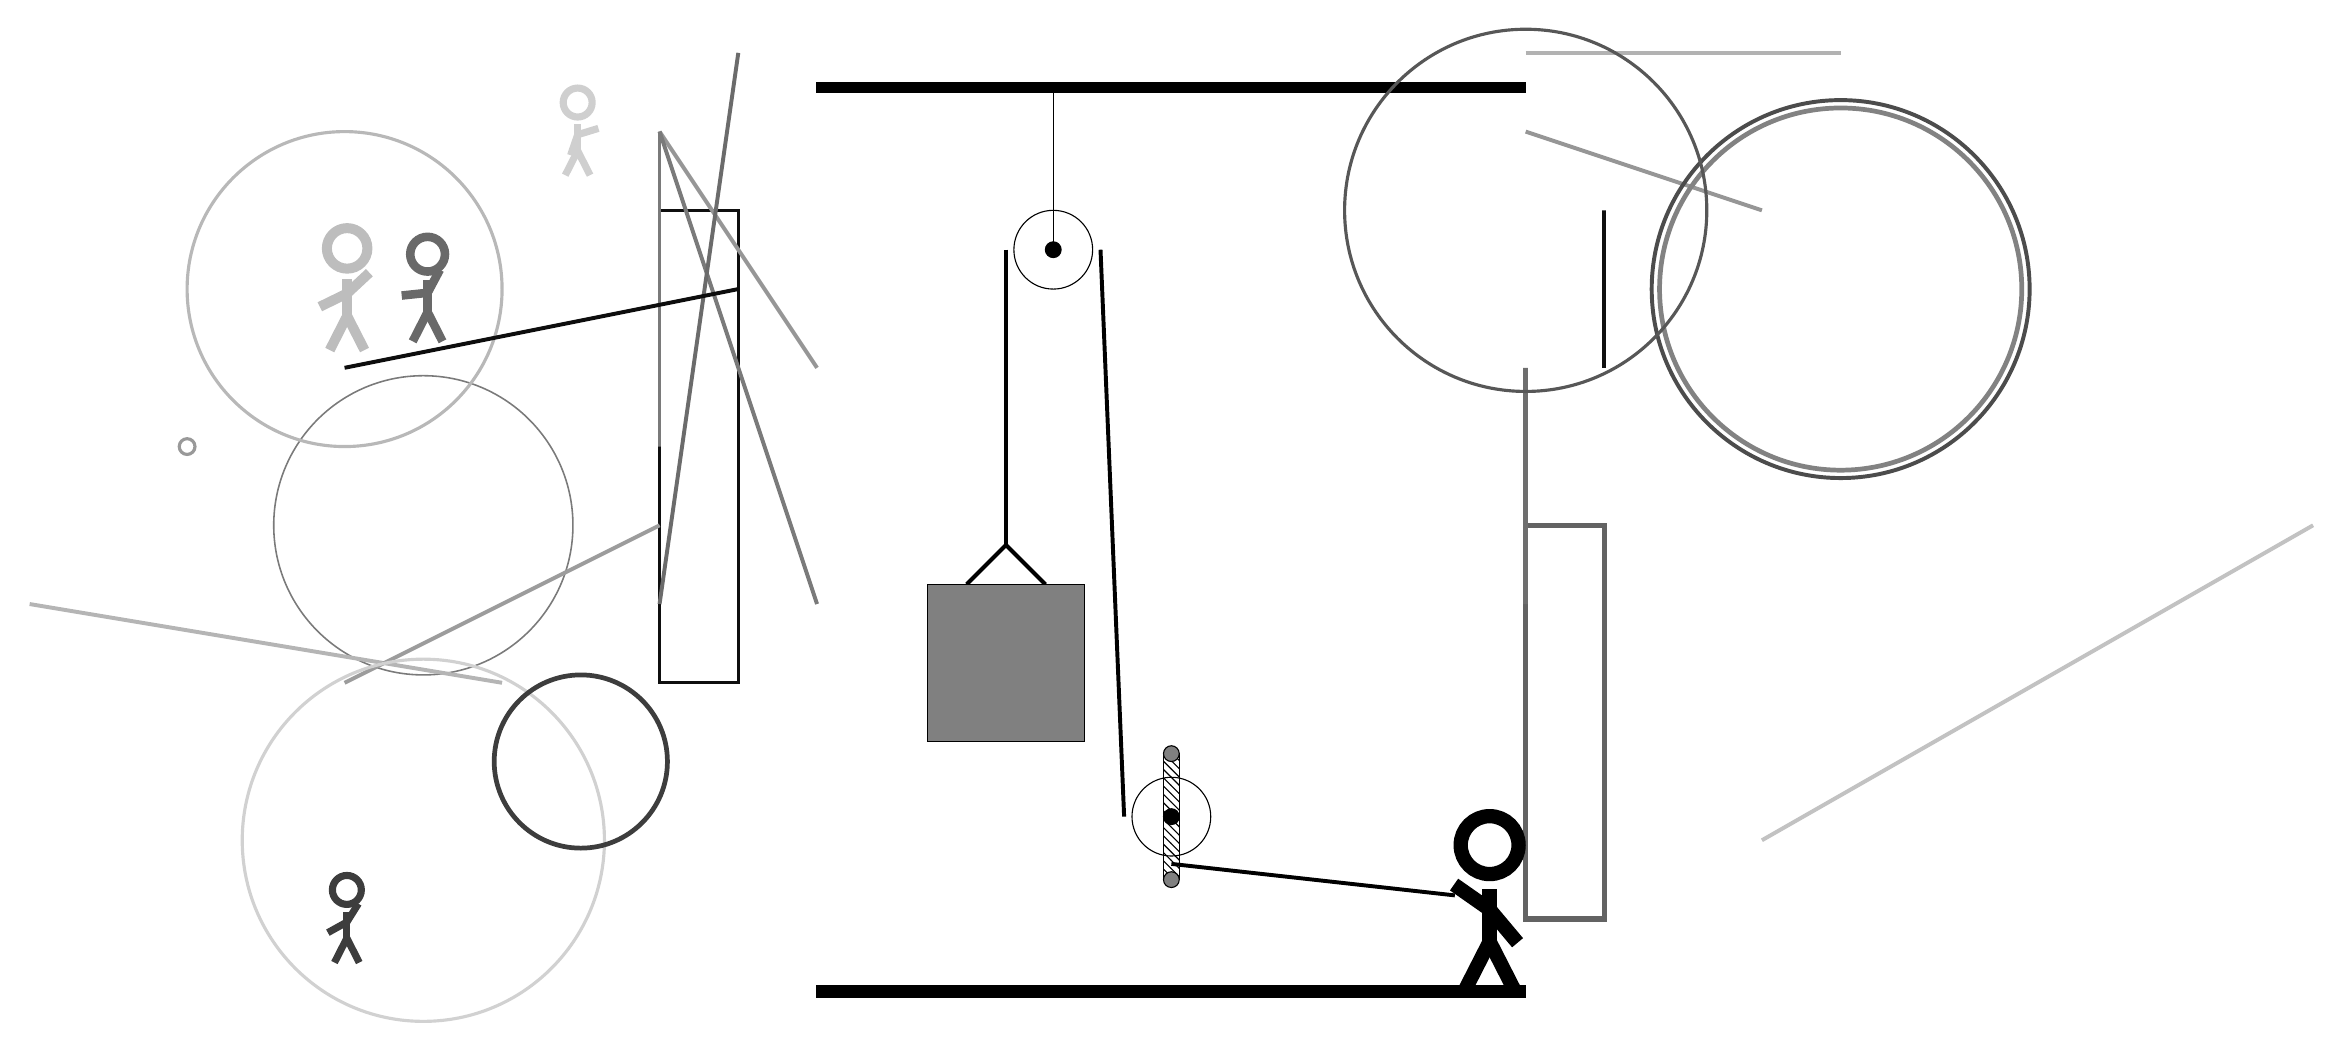
\begin{tikzpicture}
			%%%%% START %%%%%
			
			\draw[fill=black] (-2, 11.5) rectangle (7, 11.625);
			
			\draw (1, 9.5) circle (0.5);
			\draw[fill=black] (1, 9.5) circle (0.1);
			\draw (1, 11.5) -- (1, 9.5);
			
			\draw[fill=white](2.5, 2.3) circle (0.5);
			\draw[fill=black] (2.5, 2.3) circle (0.1);
			\draw[pattern=north west lines, pattern color=black] (2.4, 3.1) rectangle (2.6, 1.5);
			\draw[fill=black!50] (2.5, 3.1) circle (0.1);
			\draw[fill=black!50] (2.5, 1.5) circle (0.1);
			
			\draw[line width=0.5mm, color=black!94] (8, 8) rectangle (8, 10);
			
			\draw[line width=0.5mm, color=black!41](10, 10) -- (7, 11);
			\draw [line width=0.4mm, color=black!40](-10, 7) circle (0.1);
			\draw [line width=0.2mm, color=black!52](-7, 6) circle (1.9);
			
			\draw[line width=0.4mm, color=black!94] (-4, 4) rectangle (-3, 10);
			\draw[line width=0.5mm, color=black!29](-6, 4) -- (-12, 5);
			\draw[line width=0.5mm, color=black!39](-4, 6) -- (-8, 4);
			\draw[line width=0.7mm, color=black!61] (8, 6) rectangle (7, 1);
			\node[line width=0.6mm, color=black!19] at (-5, 11) {\Strichmaxerl[5][71][17]};
			\draw [line width=0.6mm, color=black!49](11, 9) circle (2.3);
			\node[line width=0.6mm, color=black!76] at (-8, 1) {\Strichmaxerl[5][29][58]};
			\node[line width=0.6mm, color=black!59] at (-7, 9) {\Strichmaxerl[6][6][62]};
			\draw[line width=0.4mm, color=black!52] (-4, 7) rectangle (-4, 11);
			\draw[line width=0.5mm, color=black!41](-2, 8) -- (-4, 11);
			\draw[line width=0.5mm, color=black!52](-4, 11) -- (-2, 5);
			\draw [line width=0.4mm, color=black!28](-8, 9) circle (2.0);
			\draw[line width=0.6mm, color=black!57] (7, 8) rectangle (7, 5);
			\draw [line width=0.5mm, color=black!70](11, 9) circle (2.4);
			\draw[line width=0.5mm, color=black!30](7, 12) -- (11, 12);
			\draw [line width=0.4mm, color=black!18](-7, 2) circle (2.3);
			\draw [line width=0.6mm, color=black!76](-5, 3) circle (1.1);
			\draw [line width=0.4mm, color=black!66](7, 10) circle (2.3);
			\node[line width=0.3mm, color=black!26] at (-8, 9) {\Strichmaxerl[7][26][43]};
			\draw[line width=0.5mm, color=black!58](-4, 5) -- (-3, 12);
			\draw[line width=0.5mm, color=black!24](10, 2) -- (17, 6);
			\draw[line width=0.5mm, color=black!95](-3, 9) -- (-8, 8);
			
			
			\draw[line width=0.5mm] (-0.1, 5.25) -- (0.4, 5.75) -- (0.9, 5.25);
			\draw[fill=black!50] (-0.6, 5.25) rectangle (1.4, 3.25);
			
			\draw[line width=0.5mm] (0.4, 9.5) -- (0.4, 5.75);
			\centerarc[line width=0.5mm](1, 9.5)(0:180:0.6);
			\draw[line width=0.5mm](1.6, 9.5) -- (1.9, 2.3);
			\centerarc[line width=0.5mm](2.5, 2.3)(180:270:0.6);
			\draw[line width=0.5mm](2.5, 1.7) -- (6.1, 1.3);
			
			\node at (6.5, 1.2) {\Strichmaxerl[10][-35][-50]};
			
			\draw[fill=black] (-2, 0) rectangle (7, 0.15);
			
			%%%%% END %%%%%
		\end{tikzpicture}
	\end{figure}	
\end{document}